\documentclass{tudelft-report}

%% Setting up the bibliography
% \usepackage{biblatex}
% \addbibresource{report.bib}

%% Additional packages and commands
\setlist{itemsep=-2pt} % Reducing white space in lists slightly
\renewcommand{\deg}{\si{\degree}\xspace} % Use \deg easily, everywhere
\usepackage{acronym} 
\usepackage{physics}
\usepackage{pdfpages}
% \usepackage[ruled,vlined,linesnumbered]{algorithm2e}    
\usepackage{algorithm}
\usepackage{algpseudocode}
\usepackage{dirtytalk}
\newtheorem{definition}{Definition}[section]
\newtheorem{theorem}{Theorem}[section]
\newtheorem{corollary}{Corollary}[theorem]
\newtheorem{lemma}[theorem]{Lemma}
\usepackage{makecell}
% \usepackage{landscape}
\usepackage{adjustbox}
\usepackage{booktabs}% http://ctan.org/pkg/booktabs
\newcommand{\tabitem}{~~\llap{\textbullet}~~}
\usepackage{rotating}
\usepackage{hhline}
\usepackage{multirow}
% \usepackage{hhline}
\usepackage{multicol}
\usepackage{tabularx}
\usepackage[graphicx]{realboxes}
\usepackage{colortbl}


\usepackage{parskip} %https://www.overleaf.com/learn/latex/Articles/How_to_change_paragraph_spacing_in_LaTeX
\usepackage{hyperref}
\hypersetup{
    colorlinks=true,
    linkcolor=blue,
    filecolor=magenta,      
    urlcolor=cyan,
    pdftitle={Overleaf Example},
    pdfpagemode=FullScreen,
    }
\urlstyle{same}
%%%%%%%%%%%%%%%%%%%%%%%%%%%%%
%%%%% Begin of document %%%%%
%%%%%%%%%%%%%%%%%%%%%%%%%%%%%

\begin{document}

%% Roman page numbering
\frontmatter

%% Defining the main parameters

\title{\textbf{Aggregation of Energy Flexibility}}
\subtitle{Flexibility solutions for the cities of the future} 
\author{N. K. (Nanda) Panda}
\subject{Ph.D First Year Report (23 September 2022)}
\affiliation{Delft University of Technology}

\coverimage{figures/cover.jpg} % Aspect ratio of 2:3 (portrait) recommended
\definecolor{title}{HTML}{4884d6} % Color for title

\makecover
\begin{titlepage}

\begin{center}

%% Print the title
{\makeatletter
\largetitlestyle\fontsize{45}{45}\color{black}\selectfont\@title
\makeatother}


%% Print the subtitle
{\makeatletter
\ifdefvoid{\@subtitle}{}{\bigskip\fontsize{20}{20}\selectfont\@subtitle}
\makeatother}

\bigskip
\bigskip

by

\bigskip
\bigskip

%% Print the name of the author
{\makeatletter
\largetitlestyle\fontsize{25}{25}\selectfont\@author
\makeatother}

\bigskip
\bigskip

%% Print table with names and student numbers
\setlength\extrarowheight{2pt}

\bigskip
\bigskip
    
\includegraphics[width=0.25\linewidth]{figures/IEPG logo.jpg}\\
    \textit{Intelligent Electrical Power Grids}\\
    \textbf{Faculty of Electrical Engineering, Mathematics and Computer Science}

\vfill
%% Print some more information at the bottom
\begin{tabular}{c|lcl}
\multirow{4}{*}{Go/ No-Go Commitee} & Promotor          & : & Prof.dr. P. (Peter) Palensky     \\
                                    & Co-Promotor       & : & dr. S.H. (Simon) Tindemans       \\
                                    & Member (External) & : & dr. S.J. (Stefan) Pfenninger                                 \\
                                    & Member (Internal) & : & dr. P.P. (Pedro) Vergara Barrios
\end{tabular}
\end{center}
\bigskip
\bigskip
\bigskip
\bigskip
\begin{figure*}[h]
    
\includegraphics[width=0.25\linewidth]{figures/ROBU_logo_groot (1).jpeg}
    % \caption{Caption}
    \label{fig:my_label}
\end{figure*}
\footnotesize{This PhD project is fully funded by the ROBUST project. For more information, visit their web-page at: https://tki-robust.nl/. ROBUST received funding from the \textit{MOOI 2020} Top Sector Energy subsidy programme by the Ministry of Economic Affairs and Climate Policy, executed by the Netherlands Enterprise Agency.\\
\\
\textbf{Ph.D. funding period:} 1 September 2021 till 31 August 2025}
\bigskip
\bigskip

%% Add a source and description for the cover and optional attribution for the template




%% Insert the TU Delft logo at the bottom of the page
\begin{tikzpicture}[remember picture, overlay]
    \node[above=10mm] at (current page.south) {%
        
\includegraphics[width=0.25\linewidth]{layout/tudelft/logo-black}
    };
\end{tikzpicture}

\end{titlepage}



% \chapter*{Preface}
\addcontentsline{toc}{chapter}{Preface}

\emph{A preface...}

\begin{flushright}
{\makeatletter\itshape
    \@author \\
    Delft, \monthname{} \the\year{}
\makeatother}
\end{flushright}

% \chapter*{Summary}
\addcontentsline{toc}{chapter}{Summary}

\emph{A summary...}


\tableofcontents
%\listoffigures
%\listoftables



\mainmatter

\chapter{Introduction}
\label{chapter:introduction}

\emph{An introduction... \cite{example-article}}


\chapter{About the Template}
%\label{chapter:title}

This template aims to simplify and improve the (Xe)LaTeX report template by Delft University of Technology. Some of the main features:

\begin{itemize}
  \item \textbf{Simplicity First:} A class file that has been reduced by nearly 70\% to simplify customization;
  \item \textbf{Effortless:} A careful selection of common packages to get started immediately;
  \item \textbf{Complete:} Ready-to-go when it comes to the document and file structure.
\end{itemize}

\noindent This template works with pdfLaTeX, XeLaTeX and LuaLaTeX. In order to adhere to the TU Delft house style, either XeLaTeX or LuaLaTeX is required, as it supports TrueType and OpenType fonts. BibLaTeX is used for the bibliography with as backend biber. Please visit \url{https://dzwaneveld.github.io/report} for the full documentation.

\begin{figure}[h]
    \centering
    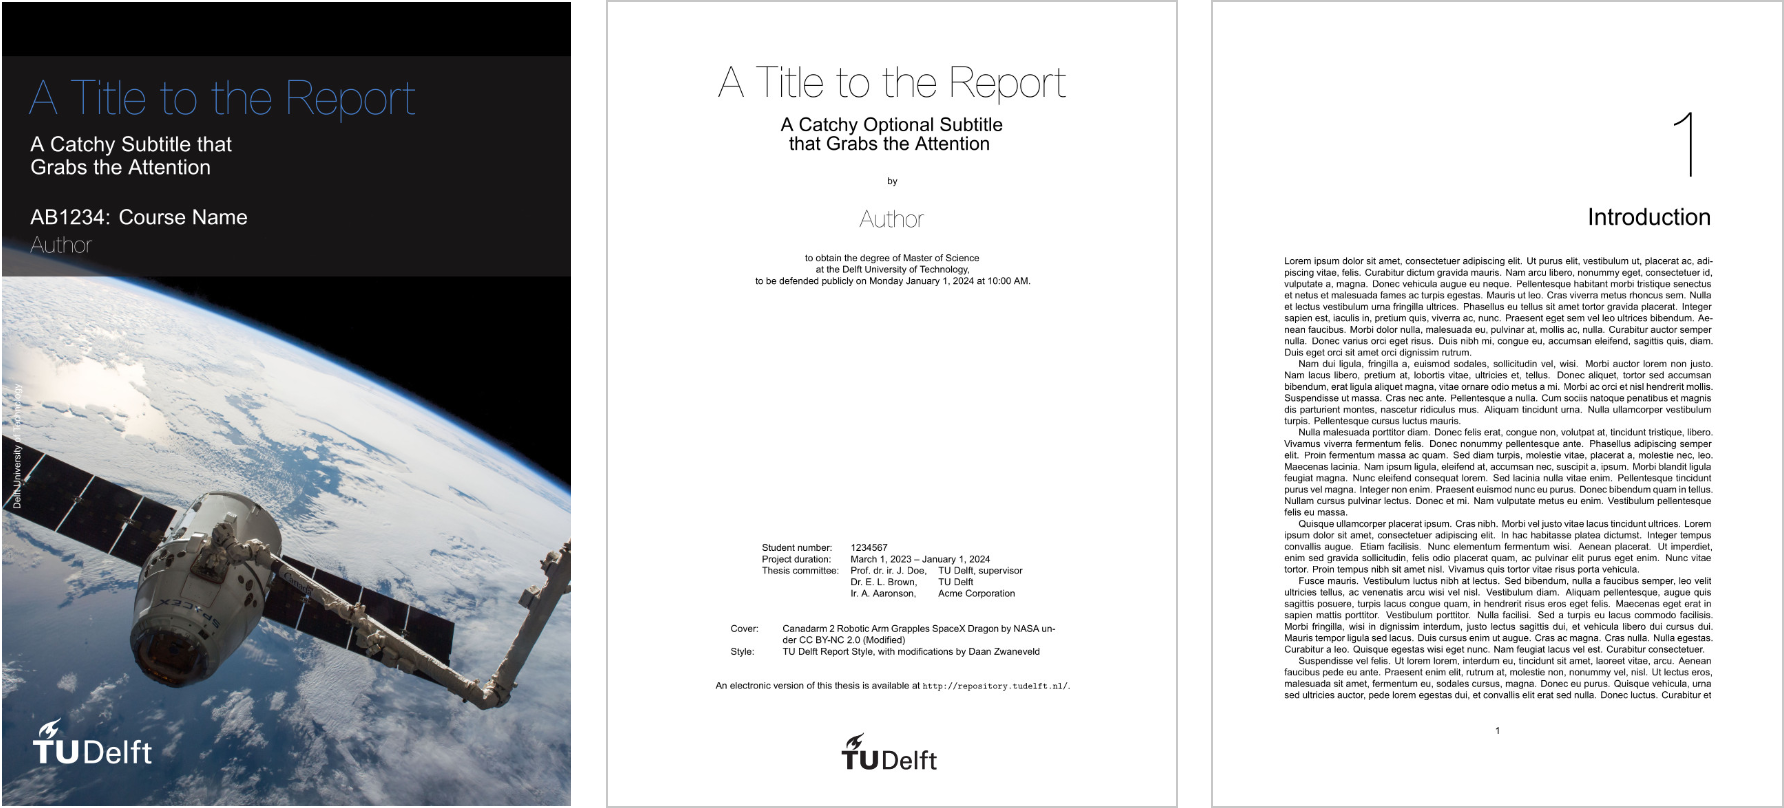
\includegraphics[width=0.95\linewidth]{figures/template.png}
    \caption{Preview of the template}
\end{figure}

\section*{License}

This template by Daan Zwaneveld is licensed under CC BY-NC 4.0. To view a copy of this license, visit \url{https://creativecommons.org/licenses/by-nc/4.0/}. No attribution is required in PDF outputs created using this template.

%\chapter{Title}
%\label{chapter:title}

%\input{mainmatter/chapter-4} % Create file to add

\chapter{Conclusion}
\label{chapter:conclusion}

\emph{A conclusion...}


%% Prevent urls running into margins in bibliography
\setcounter{biburlnumpenalty}{7000}
\setcounter{biburllcpenalty}{7000}
\setcounter{biburlucpenalty}{7000}

%% Add bibliography
\printbibliography[heading=bibintoc,title=References]

%% ----------------------------------------------------------------------
%%    Appendix (Letters for chapters)
%% ----------------------------------------------------------------------

\appendix

\chapter{Source Code Example}
%\label{chapter:title}

\emph{Adding source code to your report/thesis is supported with the package {\normalfont\texttt{listings}}. An example can be found below. Files can be added using {\normalfont\texttt{\textbackslash lstinputlisting[language=<language>]\{<filename>\}}}.}

\begin{lstlisting}[language=Python]
"""
ISA Calculator: import the function, specify the height and it will return a
list in the following format: [Temperature,Density,Pressure,Speed of Sound].
Note that there is no check to see if the maximum altitude is reached.
"""

import math
g0 = 9.80665
R = 287.0
layer1 = [0, 288.15, 101325.0]
alt = [0,11000,20000,32000,47000,51000,71000,86000]
a = [-.0065,0,.0010,.0028,0,-.0028,-.0020]

def atmosphere(h):
    for i in range(0,len(alt)-1):
        if h >= alt[i]:
            layer0 = layer1[:]
            layer1[0] = min(h,alt[i+1])
            if a[i] != 0:
                layer1[1] = layer0[1] + a[i]*(layer1[0]-layer0[0])
                layer1[2] = layer0[2] * (layer1[1]/layer0[1])**(-g0/(a[i]*R))
            else:
                layer1[2] = layer0[2]*math.exp((-g0/(R*layer1[1]))*(layer1[0]-layer0[0]))
    return [layer1[1],layer1[2]/(R*layer1[1]),layer1[2],math.sqrt(1.4*R*layer1[1])]
\end{lstlisting}

\chapter{Task Division Example}
%\label{chapter:title}

\emph{If a task division is required, a simple template can be found below for convenience. Feel free to use, adapt or completely remove.}

\begin{table}[htb]
    \setlength\extrarowheight{4pt}
    \centering
    \caption{Distribution of the workload}
    \label{tab:taskdivision}
    \begin{tabularx}{\textwidth}{lXX}
        \toprule
        & Task & Student Name(s) \\
        \midrule
        & Summary & \\
        Chapter 1 & Introduction &  \\
        Chapter 2 &  & \\
        Chapter 3 &  & \\
        Chapter * &  & \\
        Chapter * & Conclusion &  \\
        \midrule
        & Editors & \\
        & CAD and Figures & \\
        & Document Design and Layout & \\
        \bottomrule
    \end{tabularx}
\end{table}

%\input{appendix/appendix-c} % Create file to add


\bibliographystyle{IEEEtran}
\bibliography{references.bib}
%% Prevent urls running into margins in bibliography
% \setcounter{biburlnumpenalty}{7000}
% \setcounter{biburllcpenalty}{7000}
% \setcounter{biburlucpenalty}{7000}

%% Add bibliography
% \printbibliography[heading=bibintoc,title=References]

% 

%% Letters for chapters
% \appendix

% \chapter{Source Code Example}
%\label{chapter:title}

\emph{Adding source code to your report/thesis is supported with the package {\normalfont\texttt{listings}}. An example can be found below. Files can be added using {\normalfont\texttt{\textbackslash lstinputlisting[language=<language>]\{<filename>\}}}.}

\begin{lstlisting}[language=Python]
"""
ISA Calculator: import the function, specify the height and it will return a
list in the following format: [Temperature,Density,Pressure,Speed of Sound].
Note that there is no check to see if the maximum altitude is reached.
"""

import math
g0 = 9.80665
R = 287.0
layer1 = [0, 288.15, 101325.0]
alt = [0,11000,20000,32000,47000,51000,71000,86000]
a = [-.0065,0,.0010,.0028,0,-.0028,-.0020]

def atmosphere(h):
    for i in range(0,len(alt)-1):
        if h >= alt[i]:
            layer0 = layer1[:]
            layer1[0] = min(h,alt[i+1])
            if a[i] != 0:
                layer1[1] = layer0[1] + a[i]*(layer1[0]-layer0[0])
                layer1[2] = layer0[2] * (layer1[1]/layer0[1])**(-g0/(a[i]*R))
            else:
                layer1[2] = layer0[2]*math.exp((-g0/(R*layer1[1]))*(layer1[0]-layer0[0]))
    return [layer1[1],layer1[2]/(R*layer1[1]),layer1[2],math.sqrt(1.4*R*layer1[1])]
\end{lstlisting}

% \chapter{Task Division Example}
%\label{chapter:title}

\emph{If a task division is required, a simple template can be found below for convenience. Feel free to use, adapt or completely remove.}

\begin{table}[htb]
    \setlength\extrarowheight{4pt}
    \centering
    \caption{Distribution of the workload}
    \label{tab:taskdivision}
    \begin{tabularx}{\textwidth}{lXX}
        \toprule
        & Task & Student Name(s) \\
        \midrule
        & Summary & \\
        Chapter 1 & Introduction &  \\
        Chapter 2 &  & \\
        Chapter 3 &  & \\
        Chapter * &  & \\
        Chapter * & Conclusion &  \\
        \midrule
        & Editors & \\
        & CAD and Figures & \\
        & Document Design and Layout & \\
        \bottomrule
    \end{tabularx}
\end{table}

%\input{appendix/appendix-c} % Create file to add


\end{document}
